\chapter{Третій клас}

\problem
Запиши математичною мовою і~знайди значення виразів:
\begin{enumerate}
  \item Шість десятків і~п'ять взяли разом із трьома десятками і~сім.
  \item Добуток чисел 7 і~3 взяли разом із різницею чисел 8 і~4.
  \item Дочка молодша за маму на 23~роки, а~син~--- молодший на 28~років.
  Хто старший~--- дочка чи син, і~на скільки років?
  \item Від сімдесяти двох відняти добуток чисел шість і~дев'ять.
  \item Зменшити дев'яносто чотири на добуток чисел п'ять і~сім.
  \item До дванадцяти додати частку від ділення шістдесяти трьох на дев'ять.
  \item Різницю чисел 67 і~54 збільшити втричі.
  \item До частки від ділення 27 на 3 додати добуток чисел 6 і~7.
  \item Число 112 розділити на різницю чисел 82 і~78.
  \item Різницю числа 67 і добутку чисел 12 і~4 збільшити на 54.
  \item Суму числа 23 і~добутку чисел 4 і~8 зменшити в~5~разів.
  \item Суму чисел 13 і~9 розділити на 2.
  \item Від різниці чисел 16 і~7 забрати різницю чисел 11 і~3.
  \item Суму чисел 63 і~36 зменшити втричі.
  \item Добуток чисел 8 і~4 збільшити на 7.
  \item Знайти частку від ділення 24 на суму чисел 6 і~2.
\end{enumerate}


\problem
У~вірних числових рівностях хтось замалював деякі цифри:
\begin{multicols}{2}
  \begin{enumerate}
    \item $2\hiddendigit + 12 = 37$
    \item $14 + 1\hiddendigit = 33$
    \item $4\hiddendigit - \hiddendigit6 = 32$
  \end{enumerate}
\end{multicols}
Спробуй здогадатися, які цифри були замальовані.


\problem
В~БеркоШко на занятті були присутні 6~учнів і~Сашко.
В~кожного з~них у~кишені була однакова кількість цукерок.
Після того, як кожен з'їв по одній цукерці,
а~Марійка з'їла дві, всі цукерки склали до купи і~порахували.
Виявилося, що їх 20~штук.

Знайди, скільки цукерок було на початку в~кожного з~присутніх.


\problem
Намалюй:
\begin{enumerate}
  \item Чотирикутник, у~якого три сторони однакові,
  а~четверта~--- довша за інші.
  \item Чотирикутник, у~якого три сторони однакові,
  а~четверта~--- коротша за інші.
  \item Прямокутник з~трьома однаковими сторонами.
  \item Чотирикутник, у~якого всі сторони однакові, але не квадрат.
  \item Три різних чотирикутника, що можна скласти рівно з~2~клітинок;
  \item Декілька різних прямокутників, у~яких одна сторона
  на 6~см довша за іншу.
  \item Декілька різних прямокутників, у~яких одна сторона
  в~три рази довша за іншу.
  \item Прямокутник, у~якого одна сторона довша за іншу на 6~см
  і~водночас довша втричі;
\end{enumerate}


\problem
Вранці в школі в кошику було скількись яблук, частину взяли на компот,
а~решту роздали учням порівну.
Як дізнатися, скільки було яблук у~кошику, якщо відомо, скільки було учнів,
по скільки яблук вони з'їли і~скільки пішло на компот.


\problem
% TAGS: many_solutions
Банки:
\begin{enumerate}
  \item Є три банки на 2, 3, і~4~літри. Чотирилітрова банка повна соку.
  Як перелити половину у~трилітрову банку?
  \item З~повної 4-літрової банки соку необхідно розлити сік
  у~2~порожні банки, одна з~яких 2-літрова, а~друга~--- 3-літрова.
  Розлити необхідно так, щоб у~кожній опинилось по 2~літри соку.
\end{enumerate}


\problem
Побудуй:
\begin{enumerate}
  \item на аркуші в~клітинку охайний квадратик зі стороною 4~см;
  \item на аркуші в~клітинку квадратик зі стороною 2~см і~3~мм;
  \item на нелінованому аркуші квадратик зі стороною 5~см.
\end{enumerate}
Користуватися можна чим завгодно.


\problem
Міста:
\begin{enumerate}
  \item Є три міста: Київ, Одеса, Чернігів.
  Від Києва до Одеси можна доїхати двома дорогами,
  а~від Одеси до Чернігова~--- трьома.
  Знайди всі можливі варіанти проїзду від Києва до Чернігова через Одесу.
  \item Відстань від Києва до Кіровограда приблизно вдвічі більша
  за відстань від Києва до Чернігова.
  З~Києва у~Кіровоград можна доїхати приблизно за п'ять з~половиною годин.
  Як думаєш, скільки часу потрібно на подорож з~Чернігова до Кіровограда?
  \item А~від Кіровограда до Вінниці їхати приблизно стільки~ж,
  скільки від Києва до Кіровограда.
  Як думаєш, за скільки часу можна дістатися з~Чернігова до Вінниці?
\end{enumerate}


\problem
Годинник показує 7~годин і~15~хвилин.
Намалюй, уявляючи годинник із круглим циферблатом і~стрілками:
\begin{enumerate}
  \item Який час він покаже через 6~годин і~35~хвилин?
  \item Який час він покаже через 3~години і~55~хвилин?
  \item Через деякий час годинник показав 1~годину і~5~хвилин.
  Скільки часу пройшло?
\end{enumerate}
Дай відповідь на кожне з~питань і~намалюй положення стрілок на циферблаті.


\problem
% TAGS: many_solutions
Остача:
\begin{enumerate}
  \item Остача від ділення деякого числа на 8 дорівнює 5,
  а~частка дорівнює 7.
  Знайди число, яке ділили («ділене»).
  \item Остача від ділення деякого числа на 7 дорівнює 3.
  Яким може бути число, що ділили?
\end{enumerate}


\problem
Годинник відбиває час так: повні години за кількістю годин,
а~в~половину~--- один раз.
Скільки разів проб’є годинник за час навчання в~школі,
якщо заняття розпочались о~9:00, а~закінчилися~--- за 5~хвилин до 17:00.


\problem
На кукурудзі мешкала родина неймовірних зелених хробачків.
Родина була чимала, тому жити разом їм було тісно, і~неймовірні
зелені хробачки переселились на 4~сусідні кукурудзи. Усі, крім двох.
Переселилися купками по 7~неймовірних зелених хробачків на кожну кукурудзу.
Питання: скільки неймовірних зелених хробачків було в~родині до переселення?


\problem
Напиши всі можливі числа, які можна записати цифрами 2, 0, 1, 3.
Відсортуй їх від найменшого до найбільшого.


\problem
Посеред холодного південного океану біля берегів Антарктиди мешкала
зграя пінгвинів. Вдень вони любили грітися на сонечку, а~для цього
вистрибувати на велику крижину.

\begin{figure}[ht]
  \centering
  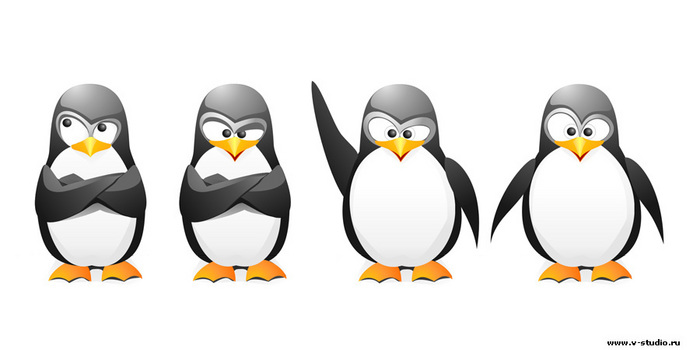
\includegraphics[width=0.8\textwidth]{3-14-1}
  \caption{Пінгвіни.}
  \label{fig:penguins}
\end{figure}

Якось у~понеділок на крижину вискочило одночасно 4~родини пінгвинів,
у~кожній родині були тато, мама і~троє маленьких миленьких пінгвинят.

У~вівторок пінгвинята так захопливо гралися на крижині,
що до них приєдналися 7~братиків-пінгвинят зі своїми батьками
і~ще одна дівчинка-пінгвинятко зі своїми дідусем і~бабусею.

А~в~середу до пінгвинів на крижині приєдналися ще 2~родини.
В~одній було двоє діточок і~мама з татом, а~в~другій~---
одне пінгвиня, мама, тато і~бабуся.

На скільки більше ставало пінгвинів на крижині кожного дня:
у~вівторок у~порівнянні з~понеділком і~в~середу в~порівнянні з~вівторком?
У~скільки разів більше пінгвинів грілося на крижині у~середу, ніж в~понеділок?


\problem
Маша йде до школи 12~хвилин, а Федько~--- 2~хвилини.
У~скільки разів більше часу потрібно Маші, щоб дійти до школи?
Скільки разів Федько встигне збігати туди й назад за той час, що дійде Маша?


\problem
\problemname{Розпізнавання фігур}

\begin{figure}[ht]
  \centering
  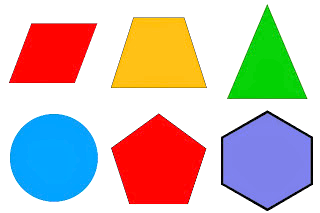
\includegraphics[width=0.8\textwidth]{3-16-1}
  \caption{Геометричні фігури.}
  \label{fig:geom-figures-recognition}
\end{figure}

Біля кожної фігури на рисунку~\ref{fig:geom-figures-recognition} познач умови,
під які вона підходить:
\begin{enumerate}
  \item має принаймні 4~кути;
  \item не всі сторони рівні;
  \item має тупий кут;
  \item є опуклим багатокутником;
  \item має увігнутий кут;
  \item є правильним багатокутником;
  \item має хоча~б 1~прямий кут;
  \item не~має кутів.
\end{enumerate}


\problem
Оля випрала рушнички і~вивісила їх сушитись у~дворі на мотузочці.
Щоб повісити 1~рушник, їй знадобилося 2~прищіпки.
Щоб повісити 3~рушники~--- 4~прищіпки (одна прищіпка тримала 2~сусідні рушники).
Скільки прищіпок знадобилось Олі, щоб розвішати 9~рушників?


\problem
Лікар накладав Федькові гіпс.
Щоб зробити один оберт навколо руки, лікар витрачав 24~см бинта.
На скільки повних обертів навколо гіпсу вистачить 5-метрового бинта?
Чи вистачить залишку бинта ще на чверть оберта?
А на півоберта?
А на дві третини?
А на три чверті?


\problem
На лавці сиділи дівчата. Раптом Маша помінялася місцями з~Томою.
А~потім Тома помінялася місцями з~Іванкою.
Тепер вони сиділи на лавці в~такому порядку: Маша, Юля, Тома та Іванка.
У~якому порядку сиділи дівчата спочатку?


\problem
\problemname{Равлик, павучок і~тарілочка}
Равлик і~павучок бігають по тарілочці,
дивись рисунок~\ref{fig:snail-spider-plate}.
Поки равлик проповзає від однієї крапочки до іншої,
павучок встигає оббігти ціле коло.

\begin{figure}[ht]
  \centering
  \begin{subfigure}{0.2\textwidth}
    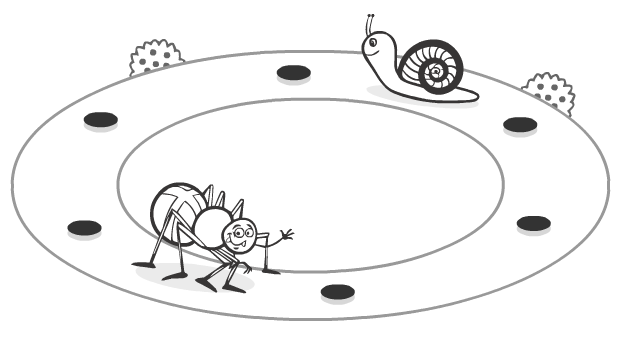
\includegraphics[width=\textwidth]{3-20-1}
  \end{subfigure}
  \quad
  \begin{subfigure}{0.4\textwidth}
    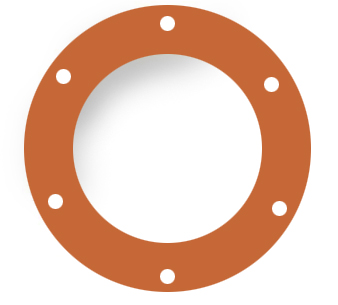
\includegraphics[width=\textwidth]{3-20-2}
  \end{subfigure}
  \quad
  \begin{subfigure}{0.2\textwidth}
    
\includegraphics[width=\textwidth]{3-20-3}
  \end{subfigure}
  \caption{Равлик, павучок і тарілочка.}
  \label{fig:snail-spider-plate}
\end{figure}

\begin{enumerate}
  \item Скільки встигне пробігти павучок за той час,
  що равлик зробить коло по тарілочці?
  \item Де опиниться равлик тоді, коли павучок пробіжить 16~кіл,
  якщо відомо, з~якої точки починав кожний з~них?
  \item Якщо павучок і~равлик побігли з~однієї точки в~різні боки,
  де вони зустрінуться?
  Намалюй відповідь якомога точніше.
  \item Де опиниться равлик, коли павучок пробіжить 42~кола, якщо відомо,
  з~якої точки починав кожний з~них і~що рухалися вони в~протилежні боки?
\end{enumerate}


\problem
Прочитай книгу Свена Нордквіста «Петсон, Фіндус і торт на іменини». Пригадай,
з~якими пригодами дідуньо намагався спекти тортик: як забракло борошна,
як збирався в~магазин, а~колесо у~веліка спустило, як загубився ключ
від столярні, як дідуньо з~котом намагалися його дістати з~колодязя,
як відволікали бика і~лізли на горище та інші.

Замалюй послідовність цих пригод.


\problem
Одного зимового дня біля школи зібралися Клим, Машка з~Платоном, Юля і~Тома,
Діма, Іванка і~Федько з~Васильком. І~почали грати у~сніжки.

Розділилися на дві команди. В~одну команду потрапили всі,
хто живе на Берківцях, а~в~іншу~--- ті, хто приїжджають\footnote{
  В нашому випадку приїжджали Клим, Юля, Тома та Діма.
}.
І~кожний заготовив собі по 8~сніжок.

\begin{enumerate}
  \item Скільки сніжок було на початку гри у~кожної команди?
  \item Діти довго перекодувалися сніжками, поки ті не закінчилися.
  Тоді хтось помітив, що рівно половина всіх сніжок влучила у~стіну школи.
  Скільки снігових кульок налипло на стіну школи?
\end{enumerate}


\problem
Софія пішла у~магазин, щоб купити для школи молока, сметани, яєць і~хліба.
Вона купила:
\begin{itemize}
  \item 3~пляшки молока по 8~грн 5~коп.
  \item 2~пачки сметани по 8~грн 64~коп.
  \item 1~десяток яєць за 9~грн 67~коп.
  \item 2~батона по 4~грн 30~коп.
\end{itemize}

Скільки всього грошей витратила Софія?


\problem
На канікули учням БеркоШко задали розв'язати приклади.
121~приклад задав Сашко, а~решту~--- Валя.
Діти зібрали всі приклади і~розділили порівну між собою.
Кожному дісталося по 48~прикладів на канікули.
Скільки прикладів задала Валя, якщо учнів було семеро?


\problem
Накресли за схемою зі сторонами світу:
\begin{multicols}{2}
  \begin{enumerate}
    \item 4~клітинки (кл.) на Сх.
    \item 1~кл. на Пн.-Сх.
    \item 1~кл. на Сх.
    \item 1~кл. на Пд.-Сх.
    \item 1~кл. на Сх.
    \item 1~кл. на Пн.-Сх.
    \item 3~кл. на Сх.
    \item 1~кл. на Пд.-Сх.
    \item 1~кл. на Сх.
    \item 1~кл. на Пн.-Сх.
    \item 1~кл. на Сх.
    \item 3~кл. на Пн.
    \item 1~кл. на Пн.-Зх.
    \item 4~кл. на Пн.
    \item 1~кл. на Сх.
    \item 1~кл. на Пн.-Зх.
    \item 4~кл. на Зх.
    \item 1~кл. на Пд.-Зх.
    \item 1~кл. на Сх.
    \item 4~кл. на Пд.
    \item 6~кл. на Зх.
    \item 2~кл. на Пн.
    \item 1~кл. на Зх.
    \item 2~кл. на Пд.
    \item 1~кл. на Пд.-Зх.
    \item 1~кл. на Пд.
    \item 3~кл. на Пд.-Зх.
  \end{enumerate}
\end{multicols}


\problem
Накресли на нелінованому аркуші прямокутник розміром $24\times16$~см.
Знайди його периметр.
Розділи його навпіл вздовж коротшої сторони.
Знайди периметр половинки.
Знову розділи навпіл і~знайди периметр четвертинки.
Знову розділи навпіл і знайди периметр восьмушки.
Продовжуй, поки прямокутники не стануть аж зовсім маленькими.
Випиши всі отримані значення периметрів в один рядок.


\problem
Замалюй і~обчисли:
\begin{enumerate}
  \item $\frac{1}{2} + \frac{1}{3}$
  \item $\frac{1}{2} - \frac{1}{3}$
  \item $\frac{2}{3} - \frac{1}{2}$
  \item $\frac{1}{3} - \frac{1}{4}$
  \item забрати від цілого третинку;
  \item до половинки додати четвертинку;
  \item скласти разом половинку і~третинку.
\end{enumerate}


\problem
Аркуш паперу склали, розрізали навпіл, потім ще навпіл і~ще, і~ще\ldots
 і~так шість разів.
Скільки утворилося шматочків?


\problem
Чи можна плавати в~басейні шириною 5~м, довжиною 10~м, глибиною 4~м,
якщо в~нього налити 15\,000~л води? А 150\,000~л?


\problem
Продовжи рядок чисел (треба здогадатися, за яким законом утворюється
наступне число з~попередніх)
\begin{enumerate}
  \item 1, 5, 9, 13, 17, 21, \ldots
  \item 57, 54, 51, 48, 45, 42, \ldots
  \item 1, 4, 10, 22, 46, 94, \ldots
  \item 1, 18, 4, 16, 7, 14, 10, 12, 13, 10, \ldots
  \item 1, 4, 3, 8, 5, 12, 7, 16, 9, \ldots
  \item 2, 6, 14, 30, 62, \ldots
  \item 2, 3, 5, 9, 17, 33, 65, \ldots
  \item 0, $\frac{1}{2}$, $1\frac{1}{2}$,
  2, $2\frac{1}{2}$, 3, $3\frac{1}{2}$, 4, \ldots
  \item 16, $15\frac{2}{3}$, $15\frac{1}{3}$, 15,
  $14\frac{2}{3}$, $14\frac{1}{3}$, 13, \ldots
  \item 1, $1\frac{3}{4}$, $2\frac{1}{2}$, $3\frac{1}{4}$,
  4, $4\frac{3}{4}$, $5\frac{1}{2}$, $6\frac{1}{4}$, \ldots
  \item 0, 1, 4, 10, 20, 35, \ldots
\end{enumerate}


\problem
Розв’яжи рівняння:
\begin{multicols}{2}
  \begin{enumerate}
    \item $(6 \cdot x - 88) : 2 - 37 = 0$
    \item $120 - (x - 8) \cdot 12 = 0$
    \item $3 \cdot (x - 2) : 5 - 15 = 0$
    \item $(x \cdot 4 - 2) : 4 + \frac{1}{4} = \frac{1}{2}$
    \item $(x \cdot \frac{1}{2} + 7) : 3 = 7$
    \item $(3 \cdot x + 1\frac{3}{4}) : 7 = 6\frac{1}{4}$
    \item $\frac{1}{4} \cdot x + (4 + 128 : 4) \cdot 2 = 78$
    \item $2 \cdot x + \frac{1}{4} = \frac{1}{2}$
    \item $(x + \frac{1}{3}) \cdot 2 = 1$
    \item $(3 \cdot x + 1) : 8 = \frac{1}{4}$
  \end{enumerate}
\end{multicols}


\problem
В~Ашані купили 5~лотків яєць.
Половину всіх яєць~--- для мешканців П'ятихаток, а~решта~--- для школи.
З~тих яєць, що віднесли до~школи, одне взяли на досліди і~залили оцтом.
А~решту~--- розділили на три дні порівну. Вийшло по 8~яєць на день.
Скільки яєць вміщається в~один лоток? 


\problem
Папай-моряк з’їв на сніданок 2~банки шпинату і~пішов у~гості до своєї
подружки Олівії. Але не зміг навіть вийти з~будинку. В~його дверях
зламався замок. А~Папаю дуже хотілося побачитися з~Олівією, тому він
з’їв ще 1~банку шпинату і~вибив двері. Потім він вирішив затулити
чимось двері, щоб злодії не~потрапили до будинку. Він знайшов неподалік
велику брилу, спробував підняти її~--- не вдалося. Тоді він з’їв ще банку
шпинату і~зміг посунути її. Поки Папай штовхав брилу до дверей, йому
довелося їсти шпинат ще тричі. І~ось, нарешті, можна вирушати до подружки.

\begin{wrapfigure}{L}{0.4\textwidth}
  \vspace{-15pt}
  \begin{center}
    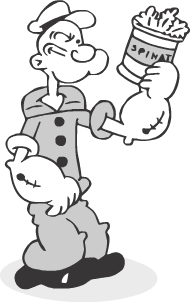
\includegraphics[width=0.4\textwidth]{3-33-1}
  \end{center}
  \vspace{-15pt}
\end{wrapfigure}

Дорогою Папай помітив двох бабусь в~автівці, які ніяк не могли рушити
з~місця. Щоб підштовхнути авто, він з’їв ще кілька баночок шпинату.

Але на цьому пригоди не скінчилися. За рогом хлопчик намагався зняти
з~дерева котеня, але його драбина була закоротка і~він ніяк не міг
дотягнутися. Тоді Папай з’їв ще шпинату, стільки, скільки й
за сніданком~--- і~підняв драбину разом із хлопчиком до котеняти.

Вже майже біля самого будинку Олівії черевик Папая заскочив у~тротуарну
решітку і~морякові знадобилось 40~хвилин і~2~банки шпинату,
або випростатися звідти.

Дзвонячи у двері Олівії, Папай зрозумів, що, якби він їв по одній
банці шпинату на день, того, що він вже з’їв сьогодні,
вистачило~б на 2~тижні.

Скільки шпинату з’їв Папай, поки йшов у~гості до Олівії, якщо в~одній
банці вміщається 400~г шпинату?
Скільки банок він з’їв, щоб підштовхнути бабусь в~автівці?


\problem
Юля до школи добирається півгодини,
третину цього часу вона їде тролейбусом, решту~--- йде пішки.
Скільки часу Юля їде тролейбусом?


\problem
Маша збиралася до БеркоШколи і~приміряла одяг.
Але довго не могла обрати, в~чому піти.
За 20~хвилин вона встигла переміряти 4~платтячка, джинси, 3~пари шкарпеток,
спідничку, кофтинку і~7~футболок.
З~якою швидкістю Маша встигала перевдягатись,
якщо кожну одежинку рахувати окремо?


\problem
Федько зробив індіанський лук і~стріли до нього.
Сів на горісі та~почав випускати стріли по мішені.
Він неперервно стріляв 17~хвилин і~за цей час випустив 51~стрілу.
А Василько тим часом бігав навколо і~шукав у~траві випущені Федьком стріли,
знайшов тільки 34.
Визнач швидкострільність Федька і~швидкість, з~якою Василько
відшукував стріли.


\problem
Іванка прийшла на день народження до Марка рівно о~шостій вечора.
На столі стояв іменинний торт, розрізаний на 24~шматочки.
Іванка з’їла один шматочок, і~цей торт їй надзвичайно сподобався.
Тоді вона пригостилася ще шматочком, і~ще одним\ldots  а далі вона вже не рахувала.
Тільки коли наїлася, зрозуміла, що сама з’їла третину торта.
Вона глянула на годинник~--- 19:20.
«О, ще купа часу!»~--- подумала Іванка і~пішла гратися з~Марком.
Але дорогою додому її зацікавило, з~якою швидкістю вона того
вечора наминала шматочки торта. Порахуй і~ти.


\problem
Минуло 20~років. Клим виріс, став археологом і~поїхав у~Південну Африку
на розкопки. Одного спекотного дня він натрапив на велику кістку
древньої істоти, ретельно викопав її, поруч була ще одна, і~ще, і~ще\ldots
До смеркання він викопав 357~кісток. І~тільки тут усвідомив, що весь
цей час працював без перерви і~навіть не~обідав. Він полишив роботу
і~повернувся в табір. Дізнайся, з~якою швидкістю Клим робив розкопки,
якщо того дня він почав роботу об 11:30, а~завершив о~пів на сьому вечора.


\problem
Діма сплів мотузку довжиною 27~метрів, з~них 9~метрів~--- тільки за сьогодні.
Яку частину мотузки сплів сьогодні Діма?


\problem
Тома читала братику Феді книжку впродовж 25~хвилин,
з~них 10~хвилин Федя сміявся.
Яку частину всього часу сміявся Томчин братик?
